\section{Introduction: Inner Product, Cauchy–Schwarz, Triangle Inequality}
\textit{Lectures 1 and 2 (Sept 10/13)}
\begin{itemize}
    \item Everything in the course will lead to Stokes' Theorem:
          \begin{equation}
              \int\limits_C \dd{W} = \int\limits_{\partial C}W
          \end{equation}
          This generalizes a well-known theorem in one-dimensional calculus, known as the Fundamental Theorem of Calculus:
          \begin{equation}
              \int\limits_{[a,b]} F'(t) = F(b) - F(a) = \int\limits_{\partial[a,b]}F
          \end{equation}
          where $\partial[a,b] = \{\underbrace{b}_{+},\underbrace{a}_{-}\}$.
    \item \textbf{Continuity in} $\mathbb{R}^n$: Recall that continuity in $\mathbb{R}$ is formally defined via $\delta-\epsilon.$ However intuitively it means that if you wiggle the input by a tiny bit, you wiggle the output by a tiny bit.

          A similar way can be used to view continuity in $\mathbb{R}^n.$
          \begin{definition}
              For $x,y\in \mathbb{R}^n$, \textbf{the standard (Euclidean) inner product} of $x$ and $y$ denoted
              \begin{equation}
                  \langle x,y\rangle = \sum_{i=1}^n x_iy_i
              \end{equation}
              The \textbf{norm squared} is defined as
              \begin{equation}
                  |x|^2 = \langle x,x\rangle
              \end{equation}
              and the \textbf{norm} of $x$ is defined:
              \begin{equation}
                  |x| = \sqrt{|x^2|} = \sqrt{\sum_{i=1}^n x_i^2}
              \end{equation}
          \end{definition}
          \begin{idea}
              There are multiple ways of defining $\mathbb{R}^n$. Some people will define it as the set of all column vectors while others define it as the set of all row vectors. In linear algebra, the distinction is important but in real analysis, this distinction is not too important.
          \end{idea}
    \item A \textbf{bilinear} function $f(x,y)$ means that the function is linear in each of the two variables. This means that
          \begin{equation}
              f(ax+by, z) = af(x,z)+bf(y,z)
          \end{equation}
          and similarly the same thing for the other parameter.
    \item A \textbf{semi-linear} function $f(x)$ is one such that
          \begin{equation}
              f(ax)=|a|f(x)
          \end{equation}
          \begin{proposition}
              If $x,y,z \in \mathbb{R}^n$ and $a,b \in \mathbb{R}$, then:
              \begin{enumerate}
                  \setcounter{enumi}{-1}
                  \item $\langle \cdot, \cdot \rangle$ is bilinear and $|\cdot |$ is semi-linear. Also note that $\langle x,y\rangle = \langle y,x\rangle.$

                  \item $|x| \ge 0$ and $|x|=0 \iff x=0$.
                  \item Cauchy–Schwarz Inequality: $|\langle x,y\rangle| \le |x||y|$ and equality holds if and only if $x,y$ are dependent.
                  \item Triangle Inequality: $|x+y| \le |x|+|y|$
                  \item Polarization Identity: $\langle x,y\rangle = \frac{|x+y|^2-|x-y|^2}{4}$
              \end{enumerate}
          \end{proposition}
          \begin{proof}
              We prove each part separately, and skip $0$:
              \begin{enumerate}
                  \item We have $|x|=\sqrt{\sum x_i^2} \ge 0$ since every $x_i^2$ is non-negative. Then $|x|=0$ if and only if $x_i=0$, i.e. $x=0$.
                  \item Consider and note that $\left||y|^2x - \langle x,y\rangle y\right|^2 \ge 0.$ This is equal to $0$ if and only if the first term (a multiple of $x$) equals the second term (a multiple of $y$), which is equivalent to $x,y$ being dependent.

                        Next, note that
                        \begin{align}
                            |s+t|^2 & = \langle s+t, s+t\rangle                                                          \\
                                    & = \langle s,s\rangle +\langle s,t\rangle + \langle t,s\rangle + \langle t,t\rangle \\
                                    & = |s|^2 + 2\langle s,t\rangle + |t|^2
                        \end{align}
                        Using this result, we can simplify the earlier expression to get that
                        \begin{align}
                            \left||y|^2x - \langle x,y\rangle y\right|^2 & = |y|^4 |x|^2 + \langle x,y\rangle^2|y|^2 - 2|y|^2 \langle x,y\rangle^2 \\
                                                                         & = |y|^2 (|y|^2|x|^2 - \langle x,y\rangle^2)
                        \end{align}
                        Since this quantity is non-negative, it follows that $|y|^2|x|^2 \ge \langle x,y\rangle^2$, which is what we wanted to show.

                        Note that there is another part regarding equality, which will not be proven in these notes.
                  \item As both $|x+y|$ and $|x|+|y|$ are nonnegative, we can square both sides. It suffices to prove that
                        \begin{align}
                            |x+y|^2                                                       & \stackrel{?}{\le} (|x|+|y|)^2             \\
                            \langle x+y, x+y\rangle                                       & \stackrel{?}{\le} |x|^2 + |y|^2 + 2|x||y| \\
                            \langle x,x\rangle + 2\langle x,y\rangle + \langle y,y\rangle & \stackrel{?}{\le} |x|^2+|y|^2+2|x||y|     \\
                            |x|^2 + 2\langle x,y\rangle + |y|^2                           & \stackrel{?}{\le} |x|^2+|y|^2 + 2|x||y|   \\
                            \langle x,y\rangle                                            & \stackrel{?}{\le} |x|\cdot |y|
                        \end{align}
                        which is true via Cauchy–Schwarz.
                        \item The proof is trivial. Expanding everything on the right hand side leads to the left hand side.
                        
                        \textit{Note:} This property is important as it tells us that if we know how to compute norms, we can compute inner products.
              \end{enumerate}
          \end{proof}
          \begin{idea}
              In the proof for 2, a weird quantity $\left||y|^2x - \langle x,y\rangle y\right|^2$ was introduced. There is actually an intuition behind it. Recall that a geometric interpretation of Cauchy-Shwarz in $\mathbb{R}^2$ can be given as follows: $\langle x,y\rangle = |x| |y| \cos\theta$ where $\theta$ is the ``angle'' between the two vectors $x,y$. This is smaller than $|x||y|$ since $\cos\theta \le 1$.
              \vspace{2mm}

              Similarly, we want to find a generalized way to express something equivalent to $\cos\theta \le 1$ in $\mathbb{R}^n$. One idea to show whether two vectors are dependent or not is to look at the separation between them, i.e. the length of the red line below.
              \begin{center}
                  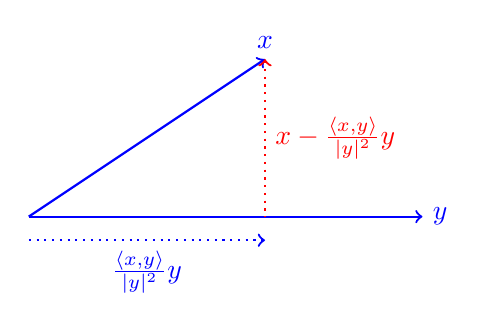
\begin{tikzpicture}
                      \draw[->,blue,thick] (0,0) -- (3,2) node[above] {$x$};
                      \draw[->,blue,thick] (0,0) -- (5,0) node[right] {$y$};
                      \draw[dotted, red, <-, thick] (3,2) -- (3,0) node[midway,right] {$x-\frac{\langle x,y\rangle}{|y|^2}y$};
                      \draw[->,blue,thick,dotted] (0,-0.3) -- (3,-0.3) node[midway,below] {$\frac{\langle x,y\rangle}{|y|^2}y$};
                  \end{tikzpicture}
              \end{center}
              Therefore, we have
              \begin{equation}
                  \left|x-\frac{\langle x,y\rangle}{|y|^2}y\right| \ge 0
              \end{equation}
              Removing the fraction gives
              \begin{equation}
                  \left||y|^2x-\langle x,y\rangle y\right| \ge 0.
              \end{equation}
          \end{idea}
\end{itemize}